\documentclass[12pt,a4paper]{article}

% ── Packages ─────────────────────────────────────────────────────────────────
\usepackage[T1]{fontenc}
\usepackage[utf8]{inputenc}
\usepackage[english]{babel}
\usepackage{lmodern}
\usepackage{amsmath,amssymb}
\usepackage{graphicx}
\usepackage{tikz}
\usepackage{circuitikz}
\usepackage{pgfplots}
\pgfplotsset{compat=1.18}
\usepackage{booktabs}
\usepackage{siunitx}
\usepackage{geometry}
\usepackage{hyperref}
\usepackage{caption}
\usepackage{subcaption}
\usepackage{float}
\usepackage{xcolor}
\usepackage{parskip}

\geometry{
  a4paper,
  top    = 25mm,
  bottom = 25mm,
  left   = 25mm,
  right  = 25mm
}

\hypersetup{
  colorlinks = true,
  linkcolor  = blue!60!black,
  citecolor  = blue!60!black,
  urlcolor   = blue!60!black,
  pdftitle   = {Buck-Boost Converter: Analysis and Design},
  pdfauthor  = {D. Turazza}
}

% ── Custom commands ───────────────────────────────────────────────────────────
\newcommand{\Vin}{V_{\mathrm{in}}}
\newcommand{\Vout}{V_{\mathrm{out}}}
\newcommand{\Iout}{I_{\mathrm{out}}}
\newcommand{\IL}{I_{L}}
\newcommand{\ILmax}{I_{L,\mathrm{max}}}
\newcommand{\ILmin}{I_{L,\mathrm{min}}}
\newcommand{\ILavg}{\langle I_L \rangle}
\newcommand{\DeltaIL}{\Delta I_L}
\newcommand{\Dduty}{D}
\newcommand{\Ts}{T_s}
\newcommand{\fs}{f_s}

% ── Title ─────────────────────────────────────────────────────────────────────
\title{%
  \textbf{Buck-Boost DC--DC Converter}\\[4pt]
  \large Steady-State Analysis: Inductor Current,\\
  Output Current, and Duty-Cycle Relationships
}
\author{claude}
\date{\today}

% ─────────────────────────────────────────────────────────────────────────────
\begin{document}
\maketitle
\tableofcontents
\newpage

% =============================================================================
\section{Introduction}
\label{sec:intro}
% =============================================================================

The \emph{buck-boost} converter is a non-isolated, single-switch DC--DC
topology that can produce an output voltage either lower or higher than its
input, with a polarity inversion.
It is widely used in battery management systems, LED drivers, and portable
power supplies where the source voltage may swing above and below the
regulated output.

This document develops the steady-state relationships between:
\begin{itemize}
  \item the duty cycle $\Dduty$,
  \item the inductor current waveform $i_L(t)$, and
  \item the DC output current $\Iout$.
\end{itemize}

Both Continuous Conduction Mode (CCM) and Discontinuous Conduction Mode
(DCM) are treated, together with the boundary condition that separates them.

% =============================================================================
\section{Circuit Topology and Operating Principle}
\label{sec:topology}
% =============================================================================

\subsection{Schematic}

The canonical non-inverting representation places the load on the negative
rail; in practice the output voltage $\Vout$ is negative with respect to the
common ground when the switch is referenced to ground.
Figure~\ref{fig:schematic} shows the standard topology.

\begin{figure}[H]
  \centering
  \begin{circuitikz}[american, scale=0.95, transform shape]
    % Ground rail
    \draw (0,0) -- (9,0);
    % Voltage source (left)
    \draw (0,0) to[V, v=$\Vin$, invert] (0,3);
    % Top rail: Vin+ to switch
    \draw (0,3) -- (1.5,3);
    % Switch S (horizontal, top rail)
    \draw (1.5,3) to[nos, l=$S$] (3,3);
    % Node A at (3,3) — junction of S, L, and D anode
    \node[circ] at (3,3) {};
    % Inductor L from node A down to ground
    \draw (3,3) to[L, l=$L$, i>^=$i_L$] (3,0);
    % Diode D from node A to output node (5,3), anode at node A
    \draw (3,3) to[D, l=$D$] (6,3);
    % Node B at (6,3) — output node
    \node[circ] at (6,3) {};
    % Capacitor C from output node to ground
    \draw (6,3) to[C, l=$C$] (6,0);
    % Load R from output node to ground
    \draw (6,3) -- (8,3);
    \draw (8,3) to[R, l=$R$] (8,0);
    \draw (8,0) -- (0,0);
    % Output voltage label
    \draw (6,3) to[open, v^=$\Vout$] (6,0);
  \end{circuitikz}
  \caption{Buck-boost converter schematic. During the ON interval, $S$
    closes and $L$ stores energy from $\Vin$; the diode $D$ is
    reverse-biased. During the OFF interval, $S$ opens and $L$ drives $D$
    into conduction, transferring energy to the output. The output voltage
    $\Vout$ is negative with respect to the input common ground.}
  \label{fig:schematic}
\end{figure}

\subsection{Two Operating Intervals}

The switch $S$ operates at frequency $\fs = 1/\Ts$ with duty cycle
$\Dduty \in (0,1)$.

\paragraph{Interval 1 — Switch ON ($0 \le t < D\Ts$).}
The switch closes; the diode is reverse-biased.
The source $\Vin$ is applied directly across the inductor:
\begin{equation}
  v_L = \Vin, \qquad
  \frac{di_L}{dt} = \frac{\Vin}{L} > 0.
  \label{eq:vL_on}
\end{equation}
Energy is stored in $L$; the output capacitor $C$ supplies the load alone.

\paragraph{Interval 2 — Switch OFF ($D\Ts \le t < \Ts$).}
The switch opens; the inductor forces the diode into conduction.
The inductor now sees $-\Vout$ (the capacitor voltage, which is negative):
\begin{equation}
  v_L = \Vout \; (<0), \qquad
  \frac{di_L}{dt} = \frac{\Vout}{L} < 0.
  \label{eq:vL_off}
\end{equation}
Energy is transferred from $L$ to the output.

% =============================================================================
\section{Voltage Conversion Ratio (CCM)}
\label{sec:voltage_ratio}
% =============================================================================

Applying the \textbf{volt-second balance} on the inductor over one switching
period (net flux change must be zero in steady state):

\begin{equation}
  \Vin \cdot D\Ts + \Vout \cdot (1-D)\Ts = 0.
\end{equation}

Solving for the conversion ratio $M(D)$:

\begin{equation}
  \boxed{M(D) = \frac{\Vout}{\Vin} = -\frac{D}{1-D}.}
  \label{eq:M_CCM}
\end{equation}

The negative sign confirms the polarity inversion.
For $D = 0.5$, $|\Vout| = \Vin$; for $D > 0.5$, the converter boosts;
for $D < 0.5$, it bucks.

% =============================================================================
\section{Inductor Current Waveform and Ripple}
\label{sec:IL_waveform}
% =============================================================================

\subsection{Peak-to-Peak Ripple}

From~\eqref{eq:vL_on}, the inductor current rises linearly during the ON
interval:
\begin{equation}
  \DeltaIL = \frac{\Vin}{L}\,D\Ts = \frac{\Vin\,D}{L\,\fs}.
  \label{eq:ripple}
\end{equation}

This can equally be expressed using the OFF interval and~\eqref{eq:vL_off}:
\begin{equation}
  \DeltaIL = \frac{|\Vout|}{L}(1-D)\Ts,
\end{equation}
which is consistent with~\eqref{eq:ripple} through~\eqref{eq:M_CCM}.

\subsection{Average Inductor Current Versus Output Current}

This is the \emph{central relationship} of this document.

In CCM, the inductor current $i_L$ flows \emph{only} through the diode
during the OFF interval, because the switch is open.
The output capacitor has zero average current in steady state; therefore
\emph{all} DC current to the load comes from the inductor through the
diode during $(1-D)\Ts$:

\begin{equation}
  \Iout
  = \frac{1}{\Ts}\int_{D\Ts}^{\Ts} i_L(t)\,dt
  = (1-D)\,\ILavg.
  \label{eq:Iout_def}
\end{equation}

Solving for the average inductor current:

\begin{equation}
  \boxed{\ILavg = \frac{\Iout}{1-D}.}
  \label{eq:ILavg_CCM}
\end{equation}

\textbf{Key insight:} Because $D \in (0,1)$, we always have
$\ILavg > \Iout$.  As $D \to 1$ the inductor must carry arbitrarily large
average current to deliver the same $\Iout$, which is a fundamental
limitation of the buck-boost topology at high duty cycles.

\subsection{Peak and Valley Values}

\begin{align}
  \ILmax &= \ILavg + \frac{\DeltaIL}{2}
          = \frac{\Iout}{1-D} + \frac{\Vin\,D}{2L\,\fs},
  \label{eq:ILmax}\\[4pt]
  \ILmin &= \ILavg - \frac{\DeltaIL}{2}
          = \frac{\Iout}{1-D} - \frac{\Vin\,D}{2L\,\fs}.
  \label{eq:ILmin}
\end{align}

The converter operates in CCM as long as $\ILmin \ge 0$, i.e.\
$\ILavg \ge \DeltaIL/2$.

% =============================================================================
\section{Boundary Between CCM and DCM}
\label{sec:boundary}
% =============================================================================

The \emph{critical} (boundary) inductance $L_B$ is defined by
$\ILmin = 0$, which gives $\ILavg = \DeltaIL/2$:

\begin{equation}
  \frac{\Iout}{1-D} = \frac{\Vin\,D}{2L_B\,\fs}.
\end{equation}

Substituting $\Vin = |\Vout|(1-D)/D$ from~\eqref{eq:M_CCM}:

\begin{equation}
  \boxed{L_B = \frac{(1-D)^2 R}{2D\,\fs},}
  \label{eq:LB}
\end{equation}

where $R = |\Vout|/\Iout$ is the load resistance.
If $L > L_B$ the converter is in CCM; if $L < L_B$ it enters DCM.

Figure~\ref{fig:iL_waveform} illustrates the inductor current waveform at
the CCM/DCM boundary and in full CCM.

\begin{figure}[H]
  \centering
  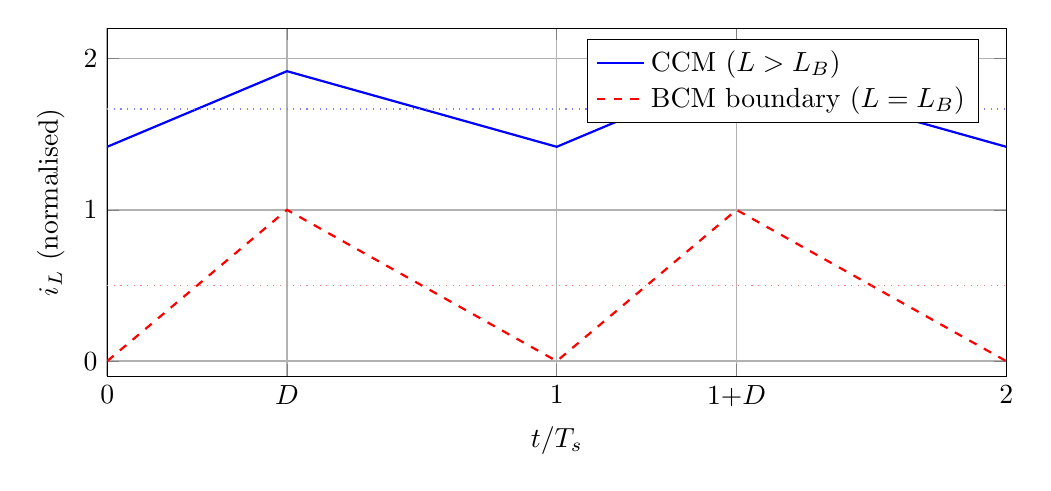
\begin{tikzpicture}
    \begin{axis}[
      width  = 13cm,
      height = 6cm,
      xlabel = {$t / T_s$},
      ylabel = {$i_L$ (normalised)},
      xmin   = 0, xmax  = 2,
      ymin   = -0.1, ymax = 2.2,
      xtick  = {0, 0.4, 1, 1.4, 2},
      xticklabels = {$0$, $D$, $1$, $1{+}D$, $2$},
      grid   = both,
      grid style = {line width=0.3pt, draw=gray!30},
      major grid style = {line width=0.5pt, draw=gray!60},
      legend pos = north east,
      legend cell align = left,
    ]
    % CCM waveform (D=0.4, ILavg=1.667, ripple=0.5)
    \addplot[blue, thick] coordinates {
      (0,   1.417)
      (0.4, 1.917)
      (1,   1.417)
      (1.4, 1.917)
      (2,   1.417)
    };
    \addlegendentry{CCM ($L > L_B$)}

    % Boundary waveform (D=0.4, ILmin=0)
    \addplot[red, thick, dashed] coordinates {
      (0,   0)
      (0.4, 1.0)
      (1,   0)
      (1.4, 1.0)
      (2,   0)
    };
    \addlegendentry{BCM boundary ($L = L_B$)}

    % Average lines
    \addplot[blue!50, thin, dotted] coordinates {(0,1.667)(2,1.667)};
    \addplot[red!50,  thin, dotted] coordinates {(0,0.5)  (2,0.5)};

    \end{axis}
  \end{tikzpicture}
  \caption{Inductor current waveforms for $D = 0.4$.  The blue trace shows
    continuous conduction mode (CCM); the red dashed trace shows the
    boundary conduction mode (BCM).  Dotted lines indicate the respective
    average values $\ILavg$.}
  \label{fig:iL_waveform}
\end{figure}

% =============================================================================
\section{Discontinuous Conduction Mode (DCM)}
\label{sec:DCM}
% =============================================================================

In DCM the inductor current reaches zero before the end of the period and
remains there for a third interval $\delta_3 \Ts$, with
$D + \delta_2 + \delta_3 = 1$.

\subsection{Voltage Conversion Ratio in DCM}

Charge balance on the output capacitor requires:

\begin{equation}
  \Iout = \frac{1}{2}\,\ILmax\,\delta_2,
  \label{eq:Iout_DCM_raw}
\end{equation}

where $\delta_2$ is the normalised duration of the diode conduction
interval.
Volt-second balance on $L$ gives $\delta_2 = D\Vin/|\Vout|$, and
$\ILmax = \Vin D \Ts / L$.
Combining:

\begin{equation}
  M_\mathrm{DCM}(D,K) = \frac{\Vout}{\Vin}
  = -\frac{1 + \sqrt{1 + 4K/D^2}}{2},
  \qquad K = \frac{2L\,\fs}{R}.
  \label{eq:M_DCM}
\end{equation}

For $K \to 0$ (light load, small $L$), $|M_\mathrm{DCM}| \to \infty$,
confirming that the output voltage tends to rise without bound in open
loop — the well-known DCM instability of the buck-boost.

\subsection{Average Inductor Current in DCM}

The average inductor current over the full period is:
\begin{equation}
  \ILavg
  = \frac{1}{2}\ILmax(D + \delta_2)
  = \frac{\Vin D \Ts}{2L}(D + \delta_2).
\end{equation}

Only the $\delta_2$ portion flows to the output, reproducing~\eqref{eq:Iout_DCM_raw}.

% =============================================================================
\section{Summary of Key Relationships}
\label{sec:summary}
% =============================================================================

Table~\ref{tab:summary} collects the most important steady-state
expressions in CCM.

\begin{table}[H]
  \centering
  \caption{Steady-state relationships of the buck-boost converter in CCM.}
  \label{tab:summary}
  \renewcommand{\arraystretch}{1.5}
  \begin{tabular}{@{} l l l @{}}
    \toprule
    \textbf{Quantity} & \textbf{Expression} & \textbf{Equation} \\
    \midrule
    Voltage gain        & $\Vout/\Vin = -D/(1-D)$              & \eqref{eq:M_CCM}    \\
    Inductor ripple     & $\DeltaIL = \Vin D / (L\fs)$         & \eqref{eq:ripple}   \\
    Average $I_L$       & $\ILavg = \Iout/(1-D)$               & \eqref{eq:ILavg_CCM}\\
    Peak $I_L$          & $\ILmax = \Iout/(1-D)+\DeltaIL/2$    & \eqref{eq:ILmax}    \\
    Valley $I_L$        & $\ILmin = \Iout/(1-D)-\DeltaIL/2$    & \eqref{eq:ILmin}    \\
    Critical inductance & $L_B = (1-D)^2 R/(2D\fs)$           & \eqref{eq:LB}       \\
    \bottomrule
  \end{tabular}
\end{table}

\subsection*{Physical interpretation of $\ILavg = \Iout/(1-D)$}

The result~\eqref{eq:ILavg_CCM} has a transparent physical origin.
Because the inductor is connected to the output \emph{only} during the
OFF interval $(1-D)\Ts$, the DC output current $\Iout$ is the time-average
of a waveform that equals $i_L$ for fraction $(1-D)$ of each period and
zero otherwise.
Therefore the DC component of $i_L$ must be scaled up by $1/(1-D)$ to
account for the duty-cycle-dependent \emph{availability} of the inductor.

This is in contrast with:
\begin{itemize}
  \item the \textbf{buck converter}, where $\ILavg = \Iout$ (inductor in
        series with the load at all times), and
  \item the \textbf{boost converter}, where $\ILavg = \Iout/(1-D)$
        with an identical formula but a different physical path — in the
        boost, the \emph{switch} current, not the inductor current, is
        pulsed; the inductor itself is always in series with the input.
\end{itemize}

% =============================================================================
\section{Design Example}
\label{sec:example}
% =============================================================================

\textbf{Specification:}
$\Vin = \SI{12}{V}$, $\Vout = -\SI{15}{V}$, $\Iout = \SI{1}{A}$,
$\fs = \SI{100}{kHz}$, maximum ripple $\DeltaIL/\ILavg \le 20\%$.

\paragraph{Duty cycle.}
From~\eqref{eq:M_CCM}:
\begin{equation*}
  \frac{15}{12} = \frac{D}{1-D}
  \;\Rightarrow\;
  D = \frac{15}{15+12} = \frac{15}{27} \approx 0.556.
\end{equation*}

\paragraph{Average inductor current.}
From~\eqref{eq:ILavg_CCM}:
\begin{equation*}
  \ILavg = \frac{1}{1-0.556} = \SI{2.25}{A}.
\end{equation*}

\paragraph{Inductance for target ripple.}
Allowed ripple: $\DeltaIL \le 0.20 \times 2.25 = \SI{0.45}{A}$.
From~\eqref{eq:ripple}:
\begin{equation*}
  L \ge \frac{\Vin\,D}{\DeltaIL\,\fs}
     = \frac{12 \times 0.556}{0.45 \times 10^5}
     \approx \SI{148}{\micro H}.
\end{equation*}
Choose $L = \SI{150}{\micro H}$.

\paragraph{Peak inductor current.}
From~\eqref{eq:ILmax}:
\begin{equation*}
  \ILmax = 2.25 + \frac{0.45}{2} = \SI{2.475}{A}.
\end{equation*}
The inductor core must be rated for at least \SI{2.48}{A} without
saturation.

\paragraph{Critical inductance check.}
From~\eqref{eq:LB}, with $R = 15/1 = \SI{15}{\Omega}$:
\begin{equation*}
  L_B = \frac{(1-0.556)^2 \times 15}{2 \times 0.556 \times 10^5}
      \approx \SI{26.6}{\micro H}.
\end{equation*}
Since $L = \SI{150}{\micro H} \gg L_B = \SI{26.6}{\micro H}$, the
converter is safely in CCM at full load.

% =============================================================================
\section{Conclusions}
\label{sec:conclusions}
% =============================================================================

The buck-boost converter inverts polarity and achieves voltage gain
$|M| = D/(1-D)$ in CCM.
The central design equation linking inductor current to output current is:

\begin{equation*}
  \ILavg = \frac{\Iout}{1-D},
\end{equation*}

which arises because the inductor delivers charge to the output only
during the OFF fraction $(1-D)$ of each period.
Consequently, the average inductor current always exceeds the output
current, and becomes increasingly large as $D \to 1$, imposing a
practical upper limit on the achievable step-up ratio in a
lossless design.
In DCM the output voltage becomes load-dependent and tends to rise
unboundedly at light load, underscoring the need for closed-loop
voltage regulation in practical implementations.

\end{document}
